\section{Validation}
\label{sec:valid}

\subsection{One pytest suite runs on three targets}
The harness uses pytest~\cite{pytest} and pySerial~\cite{pyserial}. It opens the port given by \code{--port}: a COM port for the board, or
\code{socket://127.0.0.1:PORT} for a Python mock server or for the real \code{server.c} and \code{game.c} compiled for the PC and exposed on a TCP socket.
The tests, the GUI and the board therefore share one code path. Every test starts with a known state, and the suite needs no human
action. Run with \code{python -m pytest tests --port COM9}. Results labelled \emph{PC} below were not run on the board.

\subsection{All 113 tests pass on the board; the suite detects 15 of 15 injected faults}
Table~\ref{tab:required} maps each required case of the brief to a named test. Together with the state-table and robustness tests, the board
run on the final firmware is \textbf{125 passed in 55.13~s}: 113 tests on the board (29 required and win-line tests, 18 state-table tests, 53 robustness tests and 13 AI tests) plus 12 GUI-logic tests that run on the PC against the mock (\code{ai_board_pytest.txt}). Before the AI was added the 100 original tests also passed on the board (91.96~s, \code{stage7_board_pytest.txt}). The
same tests pass on the mock and on the PC build of the real C logic (PC). The AI row covers the optional \code{NEW:AI} opponent: 13 further tests in \tn{test_ai.py} pass on the mock, on the PC build of the real C logic (113 of 113 with the original 100) and on the board (above).

A passing suite proves little unless it can fail. We injected 15 faults into the mock (for example a NACK:NOTURN that flips the turn anyway, an occupied cell that is overwritten, index 9 accepted, a stalled frame that never times out); the suite caught all 15 (PC mock, \code{stage3_mutation_check.txt}). The first run caught 14: a
fault in the 2-4-6 diagonal went unnoticed because we tested too few lines, so we added a test for all 8 lines for both players (16 cases).

\begin{table}[t]
\centering
\caption{The brief's required tests and their results on the board.}
\label{tab:required}
\scriptsize
\begin{tabular}{@{}L{3.5cm}L{3.5cm}c@{}}
\toprule
Requirement (brief, p.~4) & Test name & Result \\
\midrule
\code{CONNECT} gives \code{OK}; \code{NEW} gives empty board & \tn{test_connect_in_idle}, \tn{test_new_game_returns_empty_board} & pass \\
Legal move changes the board as expected & \tn{test_valid_move_updates_board} & pass \\
Occupied cell: \code{NACK:OCCUPIED}, board unchanged & \tn{test_occupied} & pass \\
Out of range: \code{NACK:RANGE} & \tn{test_range} & pass \\
Move after game over: \code{NACK:NOGAME} & \tn{test_x_wins_then_no_more_moves} & pass \\
Scripted win and draw & \tn{test_x_wins_...}, \tn{test_o_wins}, \tn{test_draw}, \tn{test_each_line_wins} & pass \\
AI never illegal (if implemented) & \tn{test_ai_never_loses_and_never_cheats_against_random_x}, exhaustive \tn{test_ai.c} (PC) & pass \\
\bottomrule
\end{tabular}
\end{table}

\subsection{Screenshot: the GUI shows the board's refusal and the board is unchanged}
Figure~\ref{fig:screenshot} is a screenshot of the GUI connected to the \emph{real board} on COM9 in a two-player game. The log on the right lists each frame (TX sent, RX checksum-verified reply): a move onto an occupied cell was sent and the board answered \code{NACK:OCCUPIED}, the status line shows ``That cell is already taken.'', and the board still shows X at cell 0 and O at cell 4. The GUI sends such clicks so that the refusal comes from the server, not from the client. The picture is cropped to the board and the log (the log is enlarged); no content was changed.

\begin{figure}[t]
\centering
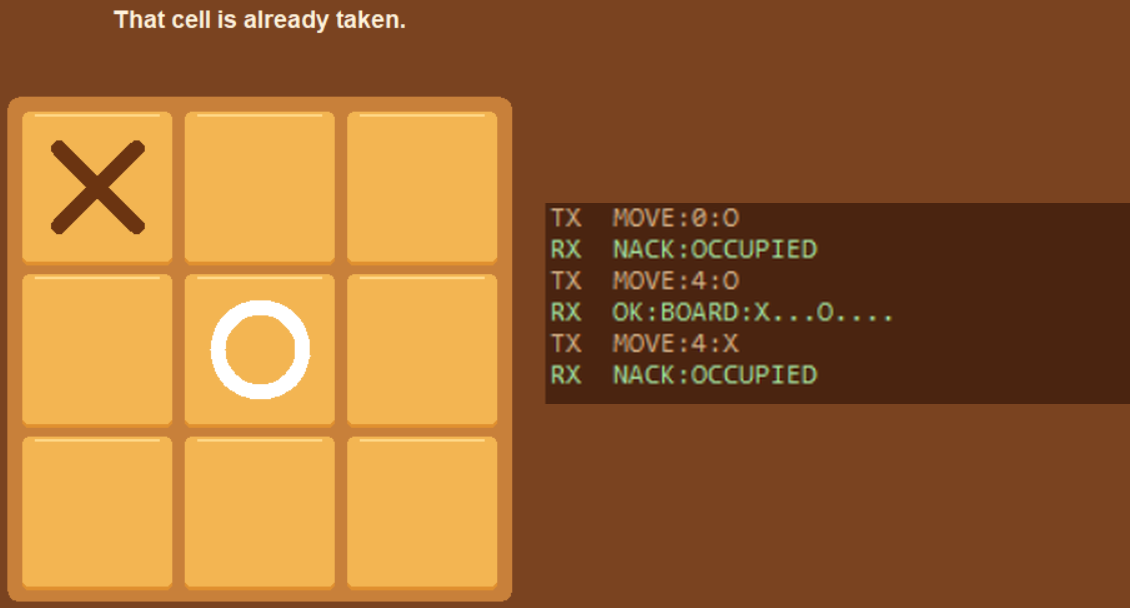
\includegraphics[width=\linewidth]{figures/gui_board_rejected.png}
\caption{GUI connected to the board (COM9): \code{NACK:OCCUPIED} twice in the log, board unchanged.}
\label{fig:screenshot}
\end{figure}

\subsection{What testing revealed}
\begin{itemize}\setlength\itemsep{0pt}
\item \emph{Timestamp underflow} in the main loop (Sec.~\ref{sec:impl}): found by code review before the first flash.
\item \emph{Diagonal gap} in the tests: found by the injected-fault run (above).
\item \emph{Fresh-clone build failure}: the Makefile's \code{mkdir build/bringup} failed when \code{build/} did not exist; we changed it to \code{mkdir -p}.
\item \emph{Read quantisation} in the test link: read latency was quantised to the 50~ms port timeout; we read \code{in_waiting} bytes instead.
\item \emph{Silent GUI sound}: \code{winsound} with \code{SND_MEMORY|SND_ASYNC} raised an error that our code swallowed; we now play from temporary WAV files. The sound plays on our PC and can be heard in the demonstration video (Sec.~\ref{sec:video}).
\item \emph{Missing ST-Link driver} on the Windows PC made the board invisible to the flash tool; installing the driver from the IDE's drivers folder fixed it.
\end{itemize}
Not tested: unplugging the cable mid-game (the GUI's lost-reply path is exercised on the mock only), UART overrun counts on the board, and the
button debounce time (30~ms is the configured value, not a measurement). The LED behaviour was observed, not measured: green when X is to move, red when O is to move, both blinking in GAME\_OVER and off after SW0 is pressed, as shown in the demonstration video; we did not time the blink, so ``2~Hz'' is the configured value only.
